%!TEX TS-program = pdflatex
%!TEX root = i3det-top.tex
%!TEX encoding = UTF-8 Unicode

\section{Introduction}
\label{sec:intro}

\subsection{IceCube Science}
\textsl{(1 page)}

\subsection{A Functional Description of the IceCube Instrument}

In order to observe astrophysical neutrinos, the primary science goal of the experiment, IceCube exploits the fact that charged particles moving through
the ice at super-luminal speed emit Cherenkov photons. An enormous detection volume is required since the cross-sections of neutrinos are small for producing secondary charged particles in interactions with ordinary matter. The glacial ice cap at the South Pole is about \SI{3}{\kilo\meter} thick and therefore predestined as operation site since it is not only offering aplenty interaction material but also a medium with unmatched high quality. 
Cherenkov light is produced in cascades of neutrino-induced muons penetrating the deep, other high-energy particles as well as generated by by cosmic-ray muons that result from cosmic-ray interactions in the atmosphere above Antarctica. 
Due to a Cherenkov photon yield of $\mathcal{O}(\num{E5})$ visible photons per \SI{}{\giga\electronvolt} of shower energy, the long optical attenuation length in South Pole ice and large-area photomultipliers (PMTs) it is possible to instrument cubic kilometers of ice with a rather wide spacing of detectors.  
The basic detection unit in IceCube in order to capture the Cherenkov light is the digital optical module or \textit{DOM} which is covered in great detail in Sec.~\ref{sec:dom}. Encapsulated in a \SI{1/2}{''} thick glass pressure sphere to withstand the extreme pressure in the deep ice, the main components of a DOM are a \SI{10}{''} PMT, embedded high-voltage generation, a flasher calibration board, and a mainboard containing the analog and digital processing circuitry for PMT pulses. 
%The transmission of the digital data is controlled by an FPGA and embedded processor hosted on the mainboard. 
The digitized data is fed to a central computing facility at the surface via a unique cable system, see Sec.~\ref{sec:cable}. 
Aspects of detector deployment and ice drilling are covered in Sec.~\ref{sec:drill-deploy}.
An overview of the data flow as well as its readout, processing and filtering are subjects of Sec.~\ref{sec:online} where we also cover the data handling, monitoring and operational performance of the observatory.
The IceCube instrument consists of three sub-detectors -- IceCube, DeepCore and IceTop -- using the same instrumentation design of embedded digital optical modules and associated surface readout. A schematic layout of the array is shown in Fig.~\ref{fig:array} 

\begin{figure}[!h]
 \centering
 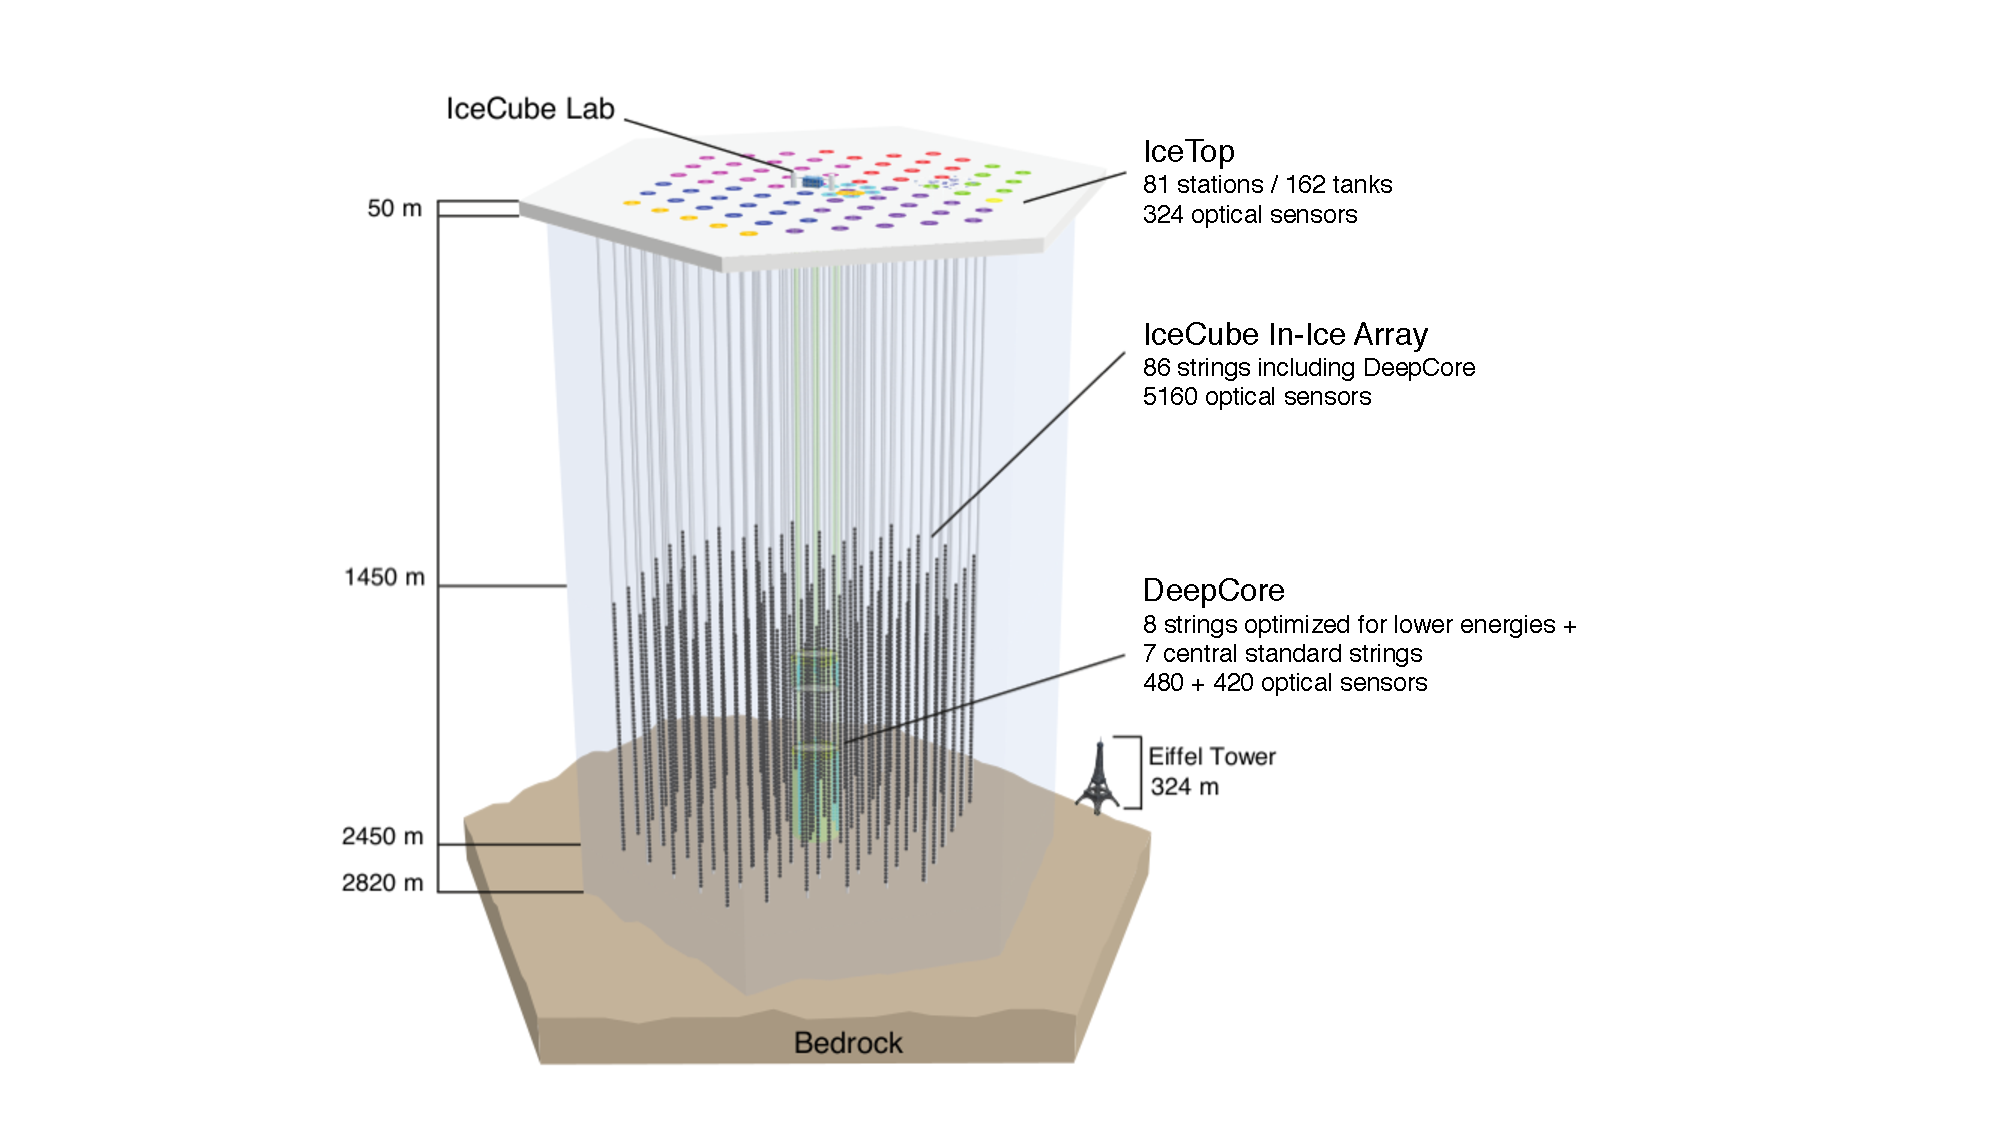
\includegraphics[width=0.8\textwidth]{graphics/intro/ArrayWSeasonsLabels_crop.pdf}
 \caption{The IceCube Neutrino Observatory with its sub-array DeepCore and the air shower array IceTop.}
 \label{fig:array}
\end{figure}


\subsubsection{IceCube}
In order to detect the Cherenkov photons emitted by charged particles traversing the ice, \num{5160} DOMs are deployed between \SI{1450}{\meter} and \SI{2450}
{\meter} below the glacial surface on \num{86} vertical strings each holding \num{60} DOMs deployed along a copper cable. The main \textit{deep-ice} 
array consists of \num{78} strings with a vertical separation of the DOMs on each string of \SI{17}{\meter}. The strings are deployed on a hexagonal grid with
\SI{125}{\meter} horizontal spacing and spanning a volume of one cubic kilometer of ice. 
This design was chosen in order to meet the primary science goal of detecting astrophysical neutrinos in the energy range of 
$\mathcal{O}(\SI{}{\tera\electronvolt}) - \mathcal{O}(\SI{}{PeV})$. The observation of these neutrinos was achieved by searching
for events that start inside the volume of IceCube and deposit more than \SI{30}{\tera\electronvolt} of energy \cite{IC3:evidence}. 
Two different event types form the standard signatures of neutrinos in IceCube.
Track-like events originate from a charged current interaction of a
high-energy muon-neutrino with a nucleus, producing a muon with
its typical Cherenkov cone along the track together with a hadronic cascade at the vertex.
An angular reconstruction of such a muon track and hence the incident neutrino direction
can reach a precision better than $ \SI{1}{\degree}$ which is confirmed by a pointing-resolution analysis
of the moon shadow \cite{IC3:moon}. Energy loss above the minimum-ionizing regime, typically $ \sim \SI{1}{\tera\electronvolt}$ in IceCube, is highly
dominated by stochastic processes resulting in large fluctuations in the amount of energy deposited for
different muons of the same energy. Another class of events are electro-magnetic or hadronic cascades from all
neutrino flavors, resulting in a spherical light deposition in the detector.
Since the total light output of such a cascade is directly proportional to its energy and the
cascades are generally well contained in the detector, the energy reconstruction for such
events is much more precise than for track-like events. The average deposited energy
resolution for both event types combined is $ \sim \SI{15}{\%}$ \cite{IC3:ereco}.


\subsubsection{DeepCore}

The remaining subset of in-ice DOMs is deployed in the deep ice below a depth of \SI{1750}{\meter} forming a denser instrumented volume. This sub-array, the DeepCore \cite{ICECUBE:DC} consists of eight specialized and closely spaced strings of sensors located around the central IceCube string. 
Its inter-string spacings are \SI{75}{\meter} and inter-DOM spacings are \SI{7}{\meter}.
Most of the PMTs in this region have \SI{35}{\%} higher quantum efficiency than the standard IceCube modules. This results in an energy threshold being about an order of magnitude below IceCube, of about \SI{10}{\giga\electronvolt}. This design is optimized for the detection of atmospheric neutrinos with energies typically in the range from \SI{10}{\giga\electronvolt} to \SI{400}{\tera\electronvolt} \cite{ICECUBE:AtmNu}.


\subsubsection{IceTop}

The air shower array IceTop \cite{ICECUBE:IceTop} consists of \num{81} Cherenkov tanks filled with clear ice that are arranged in pairs on the same, approximately \SI{125}{\meter}, triangular grid on which the in-ice array is deployed. The two tanks at each surface station are separated from each other by \SI{10}{\meter}. Each tank contains two standard IceCube DOMs. Air showers initiated in the atmosphere by cosmic rays are typically spread over a number of stations. The light generated in the tanks by the shower particles (electrons, photons, muons and hadrons) is a measure of the energy deposit of these particles in the tanks. IceTop is sensitive to primary cosmic rays of energies in the range of \SI{}{PeV} to \SI{}{EeV}  with a resolution of \SI{25}{\%} at \SI{2}{PeV}, which improves to \SI{12}{\%} above \SI{10}{PeV} \cite{IT:measurement}.




